\documentclass[]{article}
\usepackage{lmodern}
\usepackage{amssymb,amsmath}
\usepackage{ifxetex,ifluatex}
\usepackage{fixltx2e} % provides \textsubscript
\ifnum 0\ifxetex 1\fi\ifluatex 1\fi=0 % if pdftex
  \usepackage[T1]{fontenc}
  \usepackage[utf8]{inputenc}
\else % if luatex or xelatex
  \ifxetex
    \usepackage{mathspec}
  \else
    \usepackage{fontspec}
  \fi
  \defaultfontfeatures{Ligatures=TeX,Scale=MatchLowercase}
\fi
% use upquote if available, for straight quotes in verbatim environments
\IfFileExists{upquote.sty}{\usepackage{upquote}}{}
% use microtype if available
\IfFileExists{microtype.sty}{%
\usepackage{microtype}
\UseMicrotypeSet[protrusion]{basicmath} % disable protrusion for tt fonts
}{}
\usepackage[margin=1in]{geometry}
\usepackage{hyperref}
\hypersetup{unicode=true,
            pdftitle={EAS596, Homework 5},
            pdfauthor={Abhishek Kumar, Class\#1},
            pdfborder={0 0 0},
            breaklinks=true}
\urlstyle{same}  % don't use monospace font for urls
\usepackage{graphicx,grffile}
\makeatletter
\def\maxwidth{\ifdim\Gin@nat@width>\linewidth\linewidth\else\Gin@nat@width\fi}
\def\maxheight{\ifdim\Gin@nat@height>\textheight\textheight\else\Gin@nat@height\fi}
\makeatother
% Scale images if necessary, so that they will not overflow the page
% margins by default, and it is still possible to overwrite the defaults
% using explicit options in \includegraphics[width, height, ...]{}
\setkeys{Gin}{width=\maxwidth,height=\maxheight,keepaspectratio}
\IfFileExists{parskip.sty}{%
\usepackage{parskip}
}{% else
\setlength{\parindent}{0pt}
\setlength{\parskip}{6pt plus 2pt minus 1pt}
}
\setlength{\emergencystretch}{3em}  % prevent overfull lines
\providecommand{\tightlist}{%
  \setlength{\itemsep}{0pt}\setlength{\parskip}{0pt}}
\setcounter{secnumdepth}{0}
% Redefines (sub)paragraphs to behave more like sections
\ifx\paragraph\undefined\else
\let\oldparagraph\paragraph
\renewcommand{\paragraph}[1]{\oldparagraph{#1}\mbox{}}
\fi
\ifx\subparagraph\undefined\else
\let\oldsubparagraph\subparagraph
\renewcommand{\subparagraph}[1]{\oldsubparagraph{#1}\mbox{}}
\fi

%%% Use protect on footnotes to avoid problems with footnotes in titles
\let\rmarkdownfootnote\footnote%
\def\footnote{\protect\rmarkdownfootnote}

%%% Change title format to be more compact
\usepackage{titling}

% Create subtitle command for use in maketitle
\newcommand{\subtitle}[1]{
  \posttitle{
    \begin{center}\large#1\end{center}
    }
}

\setlength{\droptitle}{-2em}

  \title{EAS596, Homework 5}
    \pretitle{\vspace{\droptitle}\centering\huge}
  \posttitle{\par}
    \author{Abhishek Kumar, Class\#1}
    \preauthor{\centering\large\emph}
  \postauthor{\par}
      \predate{\centering\large\emph}
  \postdate{\par}
    \date{16/12/2018}


\begin{document}
\maketitle

\subsection{R Markdown}\label{r-markdown}

\subsection{SOLUTION 1}\label{solution-1}

\begin{center}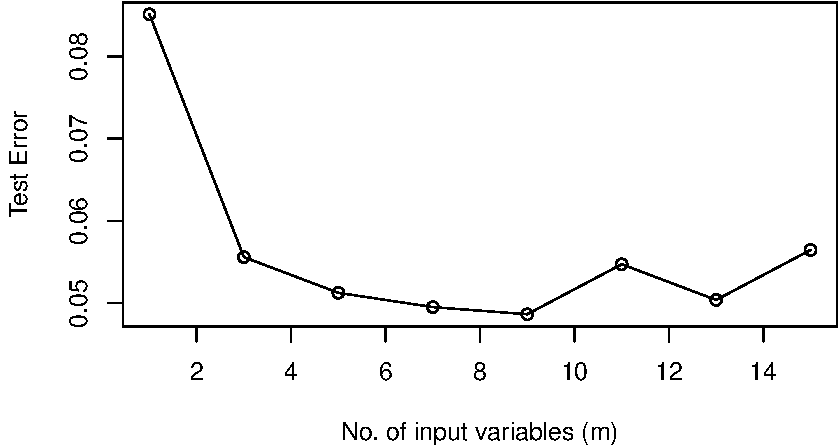
\includegraphics{HW5_Solution_files/figure-latex/unnamed-chunk-1-1} \end{center}

\begin{center}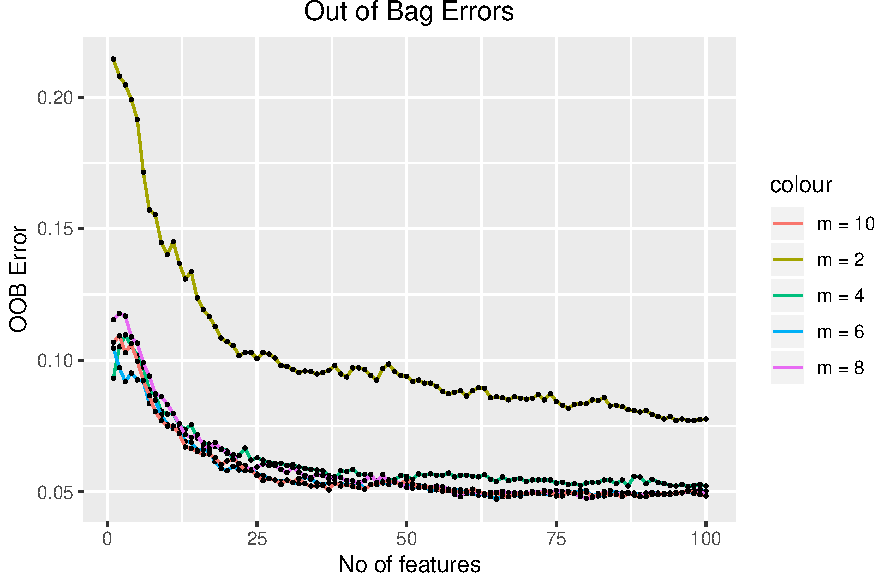
\includegraphics{HW5_Solution_files/figure-latex/unnamed-chunk-1-2} \end{center}

\subsection{SOLUTION 2}\label{solution-2}

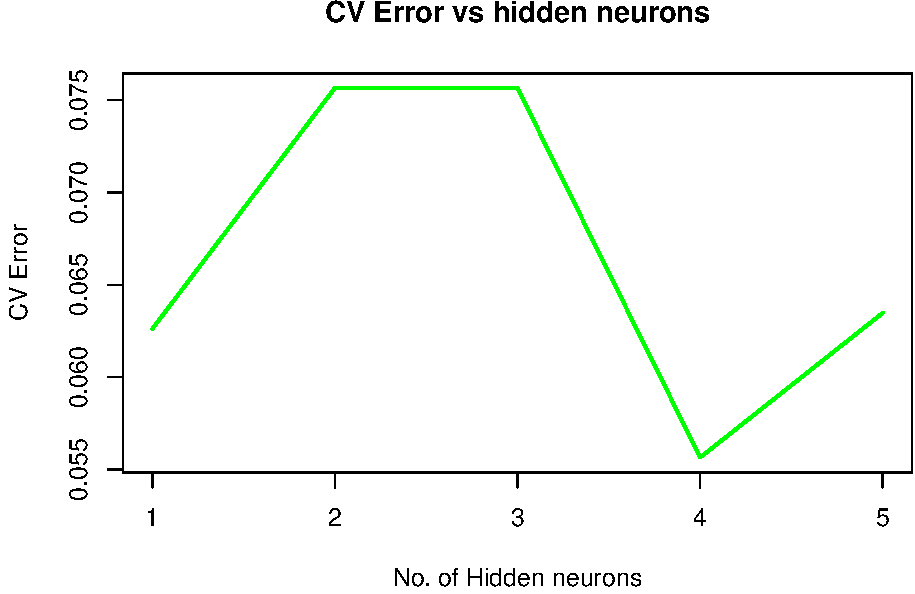
\includegraphics{HW5_Solution_files/figure-latex/unnamed-chunk-2-1.pdf}

\begin{verbatim}
## The final test error is :  0.05869565217
\end{verbatim}

As we can see using neural network with one hidden layer and 4 neurons
we get a test error of around 5.87\% which is quite less than we had
obtain using additive models like random forest. But we have to
compromise on interpretability of the model as we cannot determine which
variables were crucial in determining if the mails were spam. While
random forest implementation retains interpretability without
compromising much on accuracy. Hence, it is better to use neural
networks where we would just need accuracy and we should use other
additive models where we don't want to compromise much on
interpretability while having good accuracy.

\subsection{SOLUTION 3}\label{solution-3}

\begin{verbatim}
## Test error without any outliers :  0.08143322476
\end{verbatim}

\begin{verbatim}
## Test error when a value at 0.0628 was changed to 300 :  0.08794788274
\end{verbatim}

\begin{verbatim}
## Test error when that outlier is moved to 100 : 0.08034744843
\end{verbatim}

\begin{verbatim}
## Test error when that outlier is moved closer to 30:  0.0792616721
\end{verbatim}

\begin{verbatim}
## Test error when the outlier is moved to 3:  0.08360477742
\end{verbatim}

\begin{verbatim}
## Test error when the outlier is replaced with original value:  0.07709011944
\end{verbatim}

From the above statements we see that when just a value at 0.0628 is
changed to 300, the test error increases from 8.14\% to 8.79\% and then
when it is shrinked back to 100 the test error is 8.03\%. The effect of
outliers on the model may be more pronounced when we have several
outliers. The effect almost vanishes when the outlier is moved to 100
from 300.

\subsection{SOLUTION 4}\label{solution-4}

\subsubsection{Part(a)}\label{parta}

\begin{verbatim}
## LINEAR KERNEL ERROR, INCREASING ORDER OF COST
\end{verbatim}

\begin{verbatim}
## Train error for linear kernal : 0.1594827586 0.150862069 0.1479885057 0.1479885057 0.1465517241
\end{verbatim}

\begin{verbatim}
## Test error for linear kernal : 0.1951871658 0.1951871658 0.1951871658 0.192513369 0.2032085561
\end{verbatim}

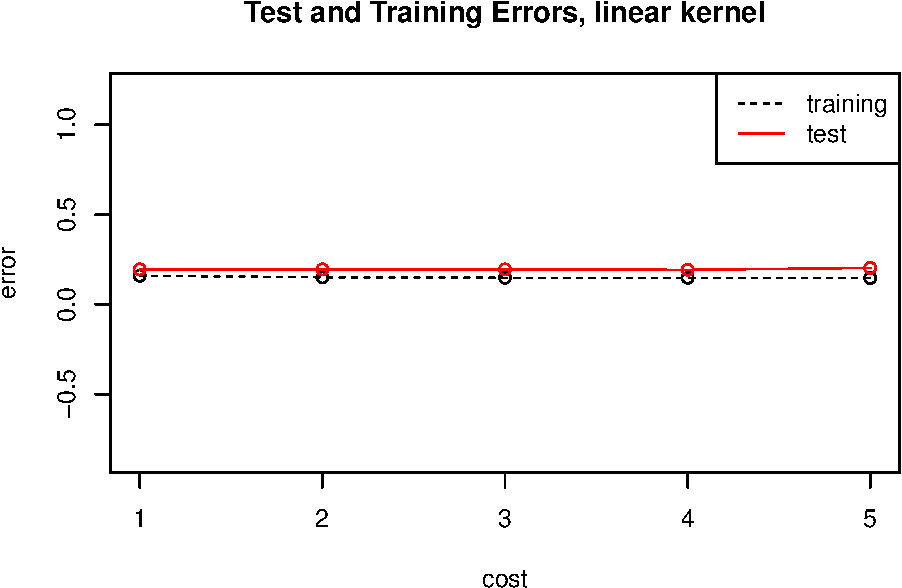
\includegraphics{HW5_Solution_files/figure-latex/unnamed-chunk-4-1.pdf}

\begin{verbatim}
## RADIAL KERNEL ERROR, INCREASING ORDER OF COST
\end{verbatim}

\begin{verbatim}
## Train error for radial kernal : 0.3850574713 0.1594827586 0.1379310345 0.1235632184 0.1206896552
\end{verbatim}

\begin{verbatim}
## Test error for radial kernal : 0.3983957219 0.192513369 0.192513369 0.2032085561 0.2032085561
\end{verbatim}

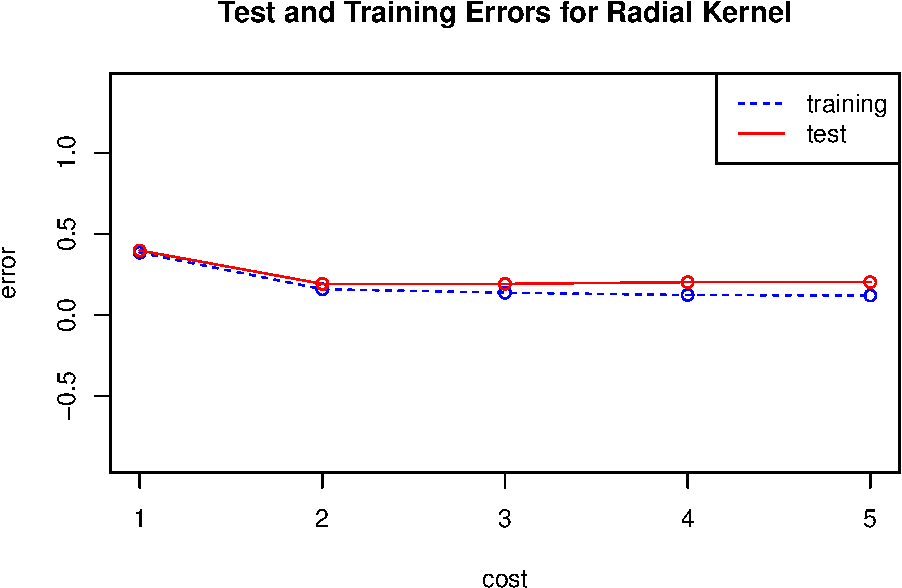
\includegraphics{HW5_Solution_files/figure-latex/unnamed-chunk-4-2.pdf}

\begin{verbatim}
## POLYNIMIAL KERNEL ERROR, INCREASING ORDER OF COST
\end{verbatim}

\begin{verbatim}
## Train error for polynomial kernal : 0.3706896552 0.2988505747 0.1781609195 0.1408045977 0.1336206897
\end{verbatim}

\begin{verbatim}
## Test error for polynomial kernal : 0.3957219251 0.3315508021 0.2112299465 0.2005347594 0.1951871658
\end{verbatim}

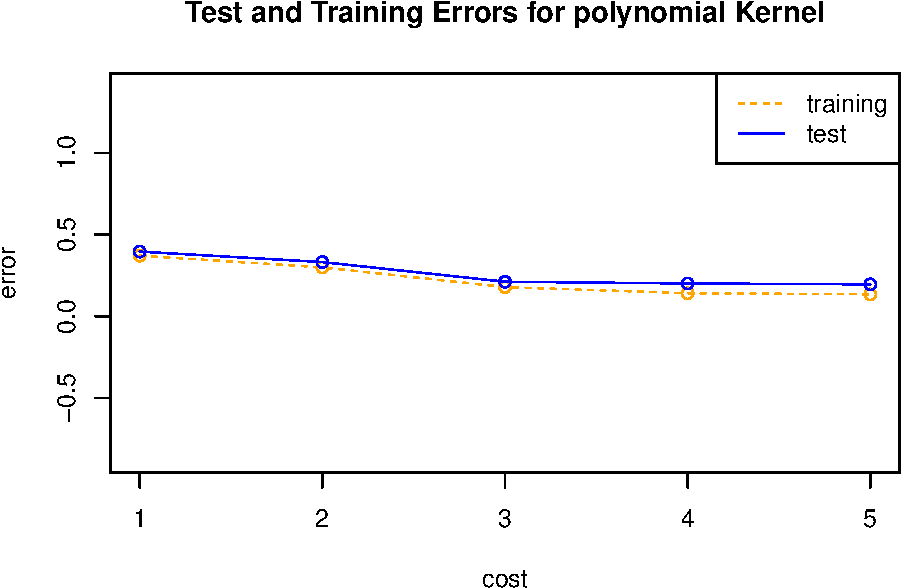
\includegraphics{HW5_Solution_files/figure-latex/unnamed-chunk-4-3.pdf}
The optimal cost for all the SVM kernel is at index 5 corresponding to
cost 10. But if we look at the plots we see that SVM with linear kernel
has minimum error even at low margin cost(index 1, cost 0.01) while SVM
with linear and polynomial kernel(order 2) has more error at margin cost
of 0.01 but they improvise when the cost is increased to 0.1 and all the
three kernels continue having almost the same error if we furthur
incerease the cost.

\subsection{SOLUTION 5}\label{solution-5}

\begin{verbatim}
## FOR GENUINE NOTES :
\end{verbatim}

\begin{verbatim}
## Importance of components:
##                              PC1       PC2       PC3      PC4       PC5
## Standard deviation     0.8289134 0.5704124 0.3978834 0.283411 0.2047993
## Proportion of Variance 0.5313800 0.2516300 0.1224300 0.062120 0.0324400
## Cumulative Proportion  0.5313800 0.7830100 0.9054400 0.967560 1.0000000
##                        PC6
## Standard deviation       0
## Proportion of Variance   0
## Cumulative Proportion    1
\end{verbatim}

\begin{verbatim}
## FOR FAKE NOTES :
\end{verbatim}

\begin{verbatim}
## Importance of components:
##                            PC1       PC2       PC3       PC4       PC5 PC6
## Standard deviation     1.24207 0.5636867 0.4038828 0.3181426 0.1617261   0
## Proportion of Variance 0.71723 0.1477200 0.0758400 0.0470600 0.0121600   0
## Cumulative Proportion  0.71723 0.8649500 0.9407800 0.9878400 1.0000000   1
\end{verbatim}

\begin{verbatim}
## FOR BOTH TYPE NOTES :
\end{verbatim}

\begin{verbatim}
## Importance of components:
##                             PC1       PC2       PC3       PC4       PC5
## Standard deviation     1.792962 0.9736636 0.4842134 0.3905824 0.1940829
## Proportion of Variance 0.698210 0.2059000 0.0509200 0.0331300 0.0081800
## Cumulative Proportion  0.698210 0.9041200 0.9550400 0.9881800 0.9963600
##                              PC6
## Standard deviation     0.1294992
## Proportion of Variance 0.0036400
## Cumulative Proportion  1.0000000
\end{verbatim}

\begin{center}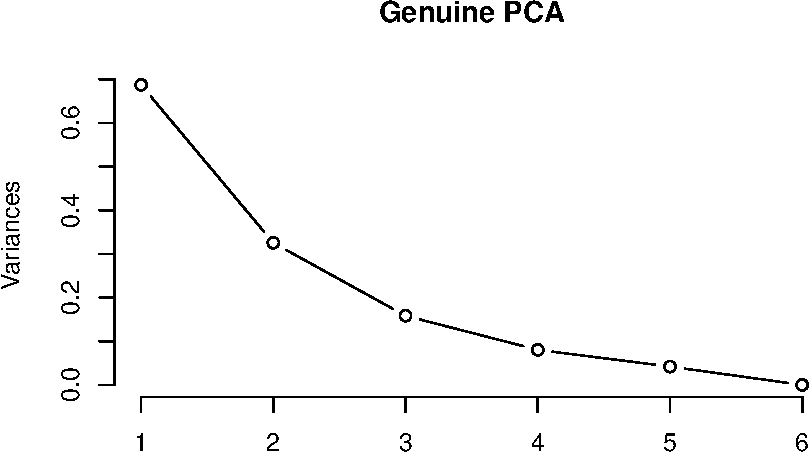
\includegraphics{HW5_Solution_files/figure-latex/unnamed-chunk-5-1} \end{center}

\begin{center}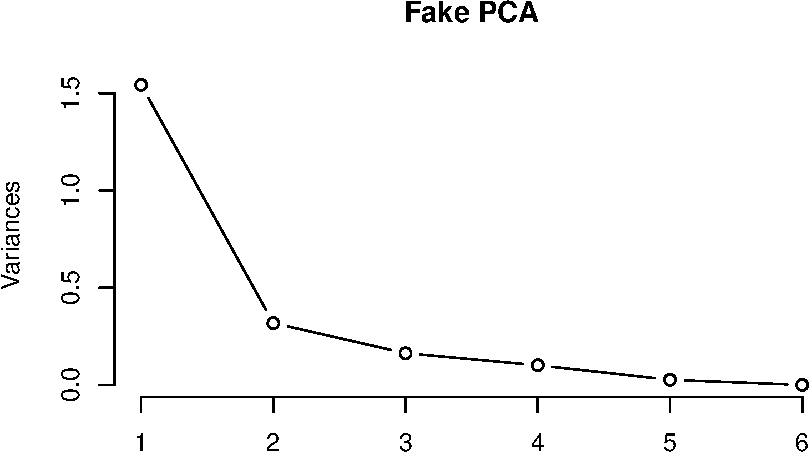
\includegraphics{HW5_Solution_files/figure-latex/unnamed-chunk-5-2} \end{center}

\begin{center}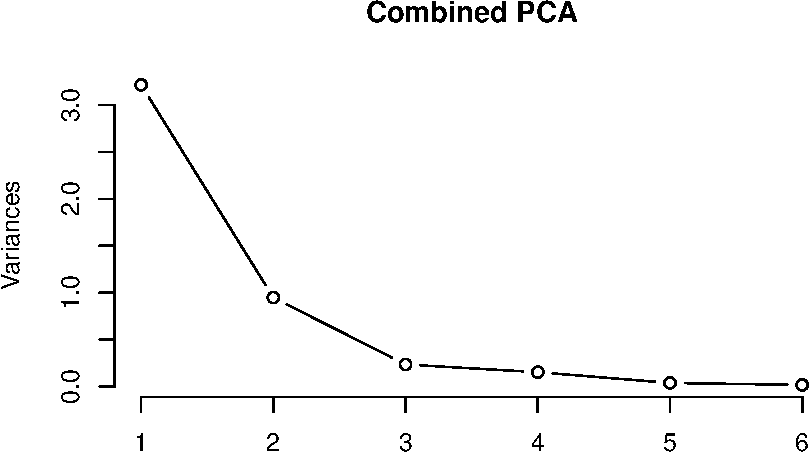
\includegraphics{HW5_Solution_files/figure-latex/unnamed-chunk-5-3} \end{center}

From the three plots above we can infer that the Genuine notes have more
number of important features as even the 5th component explains 10\% of
the variance in data while for Fake notes we can see that only two
components are dominant. For the genuine notes we select 1st 4 principle
components as it explains almost 92\% of variance in the data. And for
fake notes we only select 1st 3 principle components as it accounts for
90\% of variance in the data. This also explains that while
counterfeiting people are able to copy only some important features and
not all of them. On the combined PCA plot also we see that only only two
principle component are important and we can see this as the reason why
it is difficult to distinguish between genuine and fake notes.


\end{document}
